%\documentclass[../document.tex]{subfiles}
%\begin{document}

\chapter{Applicazione}

\section{Validazione}
Prima di presentare gli esperimenti effettuati --- e relative comparazioni fra i risultati ottenuti --- è necessario dare una breve descrizione dei procedimenti adottati per la validazione delle \textit{performance} dei vari classificatori.

\paragraph{Riconoscimento medio}
Fissato un qualsiasi metodo di classificazione multiclasse --- e un \textit{dataset} di dati pre-etichettati, da suddividere in \textit{training} e \textit{test set} --- si applichi il metodo scelto ad ogni elemento di test.
Ogni elemento $x$ avrà dunque una etichetta ``reale'' e una predetta; qualora esse non corrispondano si dice che $x$ è stato misclassificato.

Si associa al \textit{test set} una \textbf{matrice di confusione} $C$ di dimensioni $k \cdot k$, dove $C(i, j)$ contiene il numero di osservazioni di test di classe $i$, etichettate dal classificatore con $j$. $C$ fornisce quindi informazioni (qualitative e quantitative) sulle performance del metodo.
I valori sulla diagonale $C(i, i)$ rappresentano il numero di osservazioni di classe $i$ classificate correttamente.
Una misura iniziale della bontà del classificatore è data quindi dalla cosiddetta \textit{accuracy}:
\begin{equation}
	Accuracy = \frac{\sum_{i=1}^{k}{C(i, i)}}{|T|}	
	\vspace{2mm}
\end{equation}
ovvero il numero totale di osservazioni di test classificate correttamente.

\paragraph{}
La \textit{accuracy} non è l'unico indice di valutazione per un classificatore: da $C$ possono essere infatti ricavate varie misure. Per quanto riguarda gli esperimenti discussi nelle Sezioni successive, l'indice utilizzato è il \textit{riconoscimento medio}:

\begin{equation}
	\rho = \frac{\sum_{i=1}^{k}{C_\%(i, i)}}{k}	
	\vspace{2mm}
\end{equation}
dove $C_\%$ è la matrice di confusione $C$ preventivamente riportata in percentuale (dividendo ogni elemento per la somma degli elementi della sua riga).
$\rho$ è quindi la media delle percentuali di riconoscimento (simile ad \textit{accuracy}) calcolate sulle singole classi.

Quando si lavora con \textit{dataset} ``sbilanciati'' --- ovvero in cui vi è una classe predominante in numero --- la \textit{accuracy} tende a sovrastimare le reali capacità di discriminazione del classificatore: osservazioni appartenenti a classi di minore cardinalità tendono ad essere misclassificate, ciononostante la \textit{accuracy} si mantiene alta a causa dell'alto riconoscimento per la classe predominante. La scelta del riconoscimento medio come indice è un tentativo di ovviare al problema.

\paragraph{Cross-Validazione}
Un altro espediente usato al fine di ottenere misure di performance realistiche è la cosiddetta \textbf{k-fold cross-validation} (con $k = 10$).

L'idea dietro la \textit{cross-validation} è la seguente: il \textit{dataset} viene suddiviso in $k$ parti disgiunte e il procedimento consta di $k$ iterazioni; durante la $i$-esima iterazione, la $i$-esima parte ($i = 1, \, ... \, , k$) viene usata come \textit{test set} e il resto del \textit{dataset} come \textit{training set}. Si hanno quindi $k$ classificatori addestrati su sottoinsiemi del \textit{dataset} distinti. Ogni classificatore ha una matrice di confusione ed un valore di riconoscimento medio $\rho_i$.
Il valore finale di $\rho$ assunto come indice della bontà del classificatore è la media dei $\rho_i$, accompagnato dalla relativa deviazione standard dei $\rho_i$. 

\paragraph{}
La \textit{cross-validation} tende ad ``attenuare'' il valore dell'indice di riferimento, mediandolo rispetto a più scelte del \textit{training set}. Un alto valore di deviazione standard $\sigma$ associato a $\rho$ indica che le performance del metodo (fissato \textit{dataset}, kernel ed eventuali parametri) sono molto sensibili alla scelta del \textit{training set}; viceversa un valore basso di $\sigma$ indica che il metodo è abbastanza robusto in tal senso.

\paragraph{Considerazioni sui parametri}
I tre metodi discussi nel \textbf{Capitolo 3} (\textit{one-vs-all}, \textit{one-vs-one}, \textit{ibrido}) sono stati testati su vari \textit{dataset} di \textit{benchmark} e confrontati tramite $\rho$, $\sigma$ otteunti con \textit{cross-validation}.

Per quanto riguarda il metodo \textit{ibrido} (di unificazione) presentato, si ricordi che la sua applicazione dipende da un parametro di tolleranza $\epsilon$ fissato a priori. Si pone quindi il problema di scegliere opportunamente tale valore, affinché il metodo abbia buone performance.
Il procedimento adottato consiste nella ricerca esaustiva di un valore $\epsilon$ nel range $[0, 0.25]$ ottimale, cioè tale da massimizzare il valore di $\rho$. Ciò è stato realizzato facendo variare $\epsilon$ (in tale intervallo) con passo discreto (e.g. $0.01$); fissato un valore di $\epsilon = \epsilon_i$ il metodo è testato con \textit{cross-validation} (ha $\rho_i$), il valore di $\epsilon$ scelto è infine l'$\epsilon_i$ per cui si ottiene $\rho_i$ massimo.

\paragraph{}
$\epsilon$ non è inoltre l'unico parametro incontrato nel corso di questo elaborato: si ricordi e.g. il parametro $C$ nella formulazione \textit{SVM} \textit{soft-margin}, e $\sigma$ relativo al kernel \textit{RBF}.
Anche essi possono essere individuati mediante \textit{cross-validation}.

Si osservi tuttavia che l'introduzione di ulteriori parametri aumenta ``lo spazio della ricerca'' dei loro valori (e.g la coppia $(C, \epsilon)$ per cui $\rho$ è massimo).
Visto che la \textit{cross-validation} è di per sé computazionalmente dispendiosa, si è preferito trascurare tali aspetti in questa sede, posto che lo scopo della presente tesi non consiste nella classificazione ottimale dei \textit{dataset} di seguito presentati, quanto nel confrontare uniformemente i tre metodi a parità di parametri. Si è supposto quindi $C = 1$ e $\sigma_{rbf} = 1$.
La scelta di un valore per $C$ è eventualmente lasciata all'implementazione \textit{SVM} sottostante, e.g. tramite criteri euristici.

\paragraph{}
Una considerazione analoga vale per le funzioni kernel scelte:
e.g. fissato il metodo \textit{one-vs-one} con kernel quadratico, si è preferito addestrare \textit{ogni} classificatore binario (per le singole coppie di classi) con kernel quadratico.
Ovviamente al fine di massimizzare le performance è possibile selezionare tali kernel \textit{ad-hoc} (e.g. per ogni coppia di classi), in modo fortemente dipendente dal \textit{dataset} in esame. Ancora una volta, ciò che interessa non è trovare la migliore configurazione possibile per massimizzare le performance sui \textit{dataset} di \textit{benchmark}, quanto confrontare i tre metodi a parità di condizioni.

\paragraph{}
Segue che i risultati di riconoscimento di seguito presentanti sono da interpretare come \textit{migliorabili} e puramente \textit{indicativi} (del fatto che, in determinati casi, essi performano sufficientemente bene nonostante le scelte di parametri e kernel non siano ottimali). 


\section{Esperimenti e Risultati}

I \textit{dataset} scelti per l'applicazione pratica dei metodi discussi nel \textbf{Capitolo 3} sono: Ecoli\footnote{https://archive.ics.uci.edu/ml/datasets/Ecoli}, Yeast\footnote{https://archive.ics.uci.edu/ml/datasets/Yeast}, Breast Tissue\footnote{https://archive.ics.uci.edu/ml/datasets/Breast+Tissue}, ottenibili liberamente da \textit{UCI Machine Learning Repository}\footnote{https://archive.ics.uci.edu/ml/} \cite{uciml}.
Per la classificazione binaria con \textit{SVM} sono state utilizzate le funzionalità \textit{built-in} presenti in MATLAB.
A partire da esse, sono stati implementati i metodi \textit{one-vs-one}, \textit{one-vs-all}, \textit{ibrido}; più il codice necessario alla \textit{cross-validation}.

Tutti i metodi sono stati confrontati inoltre con un classificatore \textit{k-Nearest Neighbor} basato anch'esso su distanza euclidea. Un classificatore di questo tipo identifica i $k$ vicini all'osservazione $x$ --- secondo la distanza scelta --- ed assegna a $x$ l'etichetta più frequente in tali punti. Il parametro $k$ ottimale è stato ricercato con \textit{10-fold cross-validation} (così come $\epsilon$).
Le tabelle mostrano i risultati dell'applicazione dei metodi, riportando $\rho$, $\sigma$ e parametri. Si denotano con $K_1$, $K_2$, $K_3$ rispettivamente kernel lineare, quadratico e cubico ($p = 3$).

\subsection{Dataset Ecoli} %%%%%%%%%%%%%%%%%%%%%%%%%%%%%%%%%%%%
Il \textit{dataset} Ecoli contiene 336 osservazioni di 8 attributi reali che rappresentano caratteristiche biologiche di batteri della specie Escherichia Coli --- legati ai processi digestivi. L'insieme prevede un numero originario di 8 classi, tuttavia tre di esse (e i relativi esempi) sono state rimosse a causa della loro bassa cardinalità.

\begin{figure}[H] %%% grafico a barre ecoli
 	\centering	
	
	\fboxsep=0mm%padding thickness
	\fboxrule=1mm%border thickness

	\fcolorbox{border_color}{white} {
		%\includegraphics[width=\textwidth]{../img/BarEcoli.eps}
		\includegraphics[width=\textwidth]{img/BarEcoli.eps}
	}	
	\caption{Grafico a barre per il confronto dei metodi su Ecoli}
\end{figure}

\begin{center}
\begin{tabular}{ |c|c|c|c|c| } 
\hline
Metodo & Kernel & $\rho$ & $\sigma$ & Parametro \\
\hline

\multirow{1}{*}{k-NN}
& $\cdot$ & $83.8 \,\%$ & $8.1 \,\%$ & $k = 10$ \\ 
\hline

\multirow{4}{*}{one-vs-all}
& $K_1$ & $80.4 \,\%$ & $8.6 \,\%$ & $\cdot$ \\ 
& $K_2$ & $84.9 \,\%$ & $9.0 \,\%$ & $\cdot$ \\ 
& $K_3$ & $83.2 \,\%$ & $6.7 \,\%$ & $\cdot$ \\ 
& $RBF$ & $84.5 \,\%$ & $8.9 \,\%$ & $\cdot$ \\ 
\hline

\multirow{4}{*}{one-vs-one}
& $K_1$ & $84.9 \,\%$ & $5.7 \,\%$ & $\cdot$ \\ 
& $K_2$ & $85.5 \,\%$ & $8.6 \,\%$ & $\cdot$ \\ 
& $K_3$ & $82.3 \,\%$ & $7.4 \,\%$ & $\cdot$ \\ 
& $RBF$ & $84.8 \,\%$ & $5.2 \,\%$ & $\cdot$ \\ 
\hline

\multirow{4}{*}{ibrido}
& $K_1$ & $87.6 \,\%$ & $7.8 \,\%$ & $\epsilon = 0.11$ \\ 
& $K_2$ & $85.6 \,\%$ & $8.3 \,\%$ & $\epsilon = 0.09$ \\ 
& $K_3$ & $84.0 \,\%$ & $8.2 \,\%$ & $\epsilon = 0.09$ \\ 
& $RBF$ & $87.6 \,\%$ & $7.8 \,\%$ & $\epsilon = 0.11$ \\ 
\hline

\end{tabular}
\end{center}

Si può notare come, in questo caso: (a) i metodi \textit{one-vs-all} e \textit{one-vs-one} abbiano prestazioni simili, tranne nel caso lineare dove il secondo risulta più preciso (b) non solo il metodo ibrido migliora le performance di \textit{one-vs-all} (sotto qualsiasi kernel), ma risulta essere leggermente più preciso anche di \textit{one-vs-one}.
Notare inoltre come \textit{one-vs-one} nei casi lineare e RBF sia il metodo più robusto rispetto alla scelta del \textit{training set}, visto che ha minore $\sigma$.

\subsection{Dataset Yeast} %%%%%%%%%%%%%%%%%%%%%%%%%%%%%%%%%%%

\begin{figure}[H] %%% grafico a barre ecoli
 	\centering	
	
	\fboxsep=0mm%padding thickness
	\fboxrule=1mm%border thickness

	\fcolorbox{border_color}{white} {
		%\includegraphics[width=\textwidth]{../img/BarYeast.eps}
		\includegraphics[width=\textwidth]{img/BarYeast.eps}
	}	
	\caption{Grafico a barre per il confronto dei metodi su Yeast}
\end{figure}

Anche questo \textit{dataset} contiene dati di natura biologica ed in particolare caratteristiche di batteri presenti nel lievito. Di 1484 osservazioni (8 features) suddivise in 10 classi, solo le quattro classi più frequenti sono state mantenute. Nonostante ciò, la classificazione si è rivelata essere un problema abbastanza arduo su tali dati --- come è indicato nella tabella successiva (e in figura) dai bassi valori di $\rho$.

\begin{center}
\begin{tabular}{ |c|c|c|c|c| } 
\hline
Metodo & Kernel & $\rho$ & $\sigma$ & Parametro \\
\hline

\multirow{1}{*}{k-NN}
& $\cdot$ & $60.1 \,\%$ & $5.7 \,\%$ & $k = 20$ \\ 
\hline

\multirow{4}{*}{one-vs-all}
& $K_1$ & $64.8 \,\%$ & $4.8 \,\%$ & $\cdot$ \\ 
& $K_2$ & $64.7 \,\%$ & $7.6 \,\%$ & $\cdot$ \\ 
& $K_3$ & $64.5 \,\%$ & $6.8 \,\%$ & $\cdot$ \\ 
& $RBF$ & $61.8 \,\%$ & $7.1 \,\%$ & $\cdot$ \\ 
\hline

\multirow{4}{*}{one-vs-one}
& $K_1$ & $64.8 \,\%$ & $6.0 \,\%$ & $\cdot$ \\ 
& $K_2$ & $64.9 \,\%$ & $5.4 \,\%$ & $\cdot$ \\ 
& $K_3$ & $61.3 \,\%$ & $7.0 \,\%$ & $\cdot$ \\ 
& $RBF$ & $65.9 \,\%$ & $4.1 \,\%$ & $\cdot$ \\ 
\hline

\multirow{4}{*}{ibrido}
& $K_1$ & $65.1 \,\%$ & $5.3 \,\%$ & $\epsilon = 0.18$ \\ 
& $K_2$ & $65.5 \,\%$ & $7.6 \,\%$ & $\epsilon = 0.20$ \\ 
& $K_3$ & $64.9 \,\%$ & $7.5 \,\%$ & $\epsilon = 0.13$ \\ 
& $RBF$ & $63.6 \,\%$ & $6.7 \,\%$ & $\epsilon = 0.18$ \\ 
\hline

\end{tabular}
\end{center}

Si osservi comunque come i metodi basati su \textit{SVM} si comportino meglio di \textit{k-Nearest Neighbors} (con $k = 20$ opportunamente scelto). È degno di nota inoltre come il metodo ibrido non risulti meno preciso di \textit{one-vs-all}, indipendentemente dal kernel scelto.

\subsection{Dataset Breast Tissue}
Il \textit{dataset} Breast Tissue contiene 106 esempi (di 10 attributi) contenenti varie misurazioni effettuate su tessuti organici (e.g. adiposo, connettivo, etc.) al fine di identificare masse tumorali su tali tessuti. 
Poiché le 6 classi risultano ben bilanciate, nessuna è stata rimossa per il \textit{training}.
Di seguito i risultati:

\paragraph{}
\begin{center}
\begin{tabular}{ |c|c|c|c|c| } 
\hline
Metodo & Kernel & $\rho$ & $\sigma$ & Parametro \\
\hline

\multirow{1}{*}{k-NN}
& $\cdot$ & $78.3 \,\%$ & $18.9 \,\%$ & $k = 5$ \\ 
\hline

\multirow{4}{*}{one-vs-all}
& $K_1$ & $60.8 \,\%$ & $11.2 \,\%$ & $\cdot$ \\ 
& $K_2$ & $60.8 \,\%$ & $17.6 \,\%$ & $\cdot$ \\ 
& $K_3$ & $68.3 \,\%$ & $16.1 \,\%$ & $\cdot$ \\ 
& $RBF$ & $62.5 \,\%$ & $16.3 \,\%$ & $\cdot$ \\ 
\hline

\multirow{4}{*}{one-vs-one}
& $K_1$ & $69.2 \,\%$ & $14.2 \,\%$ & $\cdot$ \\ 
& $K_2$ & $65.8 \,\%$ & $19.0 \,\%$ & $\cdot$ \\ 
& $K_3$ & $67.5 \,\%$ & $20.6 \,\%$ & $\cdot$ \\ 
& $RBF$ & $74.2 \,\%$ & $21.0 \,\%$ & $\cdot$ \\ 
\hline

\multirow{4}{*}{ibrido}
& $K_1$ & $61.2 \,\%$ & $11.9 \,\%$ & $\epsilon = 0.07$ \\ 
& $K_2$ & $72.5 \,\%$ & $13.6 \,\%$ & $\epsilon = 0.08$ \\ 
& $K_3$ & $73.3 \,\%$ & $21.1 \,\%$ & $\epsilon = 0.08$ \\ 
& $RBF$ & $72.5 \,\%$ & $20.8 \,\%$ & $\epsilon = 0.20$ \\ 
\hline

\end{tabular}
\end{center}


\begin{figure}[H] %%% grafico a barre ecoli
 	\centering	
	
	\fboxsep=0mm%padding thickness
	\fboxrule=1mm%border thickness

	\fcolorbox{border_color}{white} {
		%\includegraphics[width=\textwidth]{../img/BarBreastTissue.eps}
		\includegraphics[width=\textwidth]{img/BarBreastTissue.eps}
	}	
	\caption{Grafico a barre per il confronto dei metodi su Breast Tissue}
\end{figure}

Si noti come tutti i metodi siano in questo caso particolarmente sensibili alla scelta del \textit{training set} (visti gli elevati valori di $\sigma$) --- \textit{k-NN} incluso --- ciò suggerisce che tale problematica sia inerente ai dati piuttosto che al metodo scelto. È evidente come nel caso lineare \textit{one-vs-one} sia significativamente più preciso di \textit{one-vs-all}, e come con kernel quadratico e cubico il metodo ibrido sia più preciso del primo. Con kernel RBF, invece, il metodo ibrido si avvicina comunque a \textit{one-vs-one}, migliorando le prestazioni di \textit{one-vs-all}.

Notare inoltre come, a dispetto della sua semplicità, \textit{k-NN} abbia in questo caso prestazioni migliori di tutti i metodi basati su \textit{SVM}, indipendentemente dal kernel (ciò potrebbe non essere più vero scegliendo adeguatamente i kernel \textit{ad-hoc}, comunque --- per quanto detto nella sezione precedente).
\section{Conclusioni}

A partire dagli esperimenti effettuati, sembra lecito dedurre le seguenti conclusioni:

\begin{itemize}
\item{il metodo \textit{one-vs-one} raggiunge in genere prestazioni maggiori di \textit{one-vs-all}, specialmente a parità di kernel lineare e RBF;}

\item{sotto kernel cubico le prestazioni di \textit{one-vs-one} tendono invece ad abbassarsi;}

\item{in quasi tutti i casi esaminati, il metodo ibrido è in grado di avvicinarsi alle prestazioni di \textit{one-vs-one} e a volte di superarle.}
\end{itemize}
 
Il criterio nel \textbf{Capitolo 3}, pur essendo abbastanza semplice, consente in determinati casi di migliorare la precisione di \textit{one-vs-all} pagando un piccolo prezzo in termini computazionali --- ovvero introducendo una ricerca lineare in $k$; per un totale di $O(2k +1)$ --- ma rimanendo comunque più efficiente di \textit{one-vs-one} durante il test, almeno in linea teorica (non si considera né la complessità di calcolo del kernel scelto né il numero di vettori di supporto).

Ciò suggerisce, per quanto riguarda eventuali sviluppi futuri, che sia possibile lavorare ulteriormente in questa direzione, cercando di trovare un compromesso fra \textit{one-vs-all} e \textit{one-vs-one} formulando criteri più sofisticati e raffinati.

%\end{document}